%% Based on a TeXnicCenter-Template by Gyorgy SZEIDL.
%%%%%%%%%%%%%%%%%%%%%%%%%%%%%%%%%%%%%%%%%%%%%%%%%%%%%%%%%%%%%

%------------------------------------------------------------
%
\documentclass{article}%
%Options -- Point size:  10pt (default), 11pt, 12pt
%        -- Paper size:  letterpaper (default), a4paper, a5paper, b5paper
%                        legalpaper, executivepaper
%        -- Orientation  (portrait is the default)
%                        landscape
%        -- Print size:  oneside (default), twoside
%        -- Quality      final(default), draft
%        -- Title page   notitlepage, titlepage(default)
%        -- Columns      onecolumn(default), twocolumn
%        -- Equation numbering (equation numbers on the right is the default)
%                        leqno
%        -- Displayed equations (centered is the default)
%                        fleqn (equations start at the same distance from the right side)
%        -- Open bibliography style (closed is the default)
%                        openbib
% For instance the command
%           \documentclass[a4paper,12pt,leqno]{article}
% ensures that the paper size is a4, the fonts are typeset at the size 12p
% and the equation numbers are on the left side
%
\usepackage{amsmath}%
\usepackage{amsfonts}%
\usepackage{amssymb}%
\usepackage{graphicx}
%-------------------------------------------
\newtheorem{theorem}{Theorem}
\newtheorem{acknowledgement}[theorem]{Acknowledgement}
\newtheorem{algorithm}[theorem]{Algorithm}
\newtheorem{axiom}[theorem]{Axiom}
\newtheorem{case}[theorem]{Case}
\newtheorem{claim}[theorem]{Claim}
\newtheorem{conclusion}[theorem]{Conclusion}
\newtheorem{condition}[theorem]{Condition}
\newtheorem{conjecture}[theorem]{Conjecture}
\newtheorem{corollary}[theorem]{Corollary}
\newtheorem{criterion}[theorem]{Criterion}
\newtheorem{definition}[theorem]{Definition}
\newtheorem{example}[theorem]{Example}
\newtheorem{exercise}[theorem]{Exercise}
\newtheorem{lemma}[theorem]{Lemma}
\newtheorem{notation}[theorem]{Notation}
\newtheorem{problem}[theorem]{Problem}
\newtheorem{proposition}[theorem]{Proposition}
\newtheorem{remark}[theorem]{Remark}
\newtheorem{solution}[theorem]{Solution}
\newtheorem{summary}[theorem]{Summary}
\newenvironment{proof}[1][Proof]{\textbf{#1.} }{\ \rule{0.5em}{0.5em}}

\begin{document}

\begin{flushleft}
\textbf{Course:} CSC520, Introduction to Artificial Intelligence\\
\textbf{Homework 2}\\
\textbf{Student: Xusheng Xiao} \\
\textbf{Unity ID: xxiao2} \\
\textbf{Email: xxiao2@ncsu.edu}
\end{flushleft}

\noindent{\hrulefill}

\bigskip

\begin{enumerate}
	\item \textbf{ (34 points) Consider the following English sentences.:}
	\begin{enumerate}
	\item John is a lawyer.
    \item Lawyers are rich.
    \item Rich people have big houses.
    \item Big houses are a lot of work to maintain.
    \item John has a house.
	\end{enumerate}
     
    Answer the following questions:
     \begin{enumerate}
	\item (10 points) Convert the sentences into first order predicate logic. Use the following lexicon: \\
	Functions: $houseof(X)$ -- the house of $X$ \\
	Predicates: $lawyer(X)$ -- $X$ is a lawyer\\
            $rich(X)$ -- $X$ is rich \\
            $big(X)$ -- $X$ is big \\
            $lotofwork(X)$ -- $X$ is a lot of work \\
            $house(X, Y)$ -- the owner of house $X$ is $ Y$\\
        \begin{enumerate}
		\item $ lawyer(john) $
		\item $ \forall X (lawyer(X) \Rightarrow rich(X)) $
		\item $ \forall X (rich(X) \Rightarrow house(houseof(X)) \wedge big(houseof(X)) ) $
		\item $ \forall X (big(houseof(X)) \Rightarrow lotofwork(houseof(X))) $
		\item $ house(houseof(john)) $
		\end{enumerate} 
    \item (12 points) Convert the logic statements into CNF.
    	\begin{enumerate}
		\item $ lawyer(john) $
		\item $ \neg lawyer(X1) \vee rich(X1) $
		\item $ \neg rich(X2) \vee house(houseof(X2)) $ 
		\item $ \neg rich(X3) \vee big(houseof(X3)) $
		\item $ \neg big(houseof(X4)) \vee lotofwork(houseof(X4)) $
		\item $ house(houseof(john)) $
		\end{enumerate}
	\item (12 points) Using resolution, prove that "John's house is a lot of work to maintain." \\
	Conclusion: $ house(houseof(john)) \wedge lotofwork(houseof(john))$\\
		------------------------------------------------\\
		Negated conclusion:  \\
		1. $ \neg house(houseof(john)) \vee \neg lotofwork(houseof(john))$ \\
		------------------------------------------------\\
		\begin{tabular}{c|p{8cm}|l}
		2. & $ rich(john) $ &  $i + ii \lbrace john / X \rbrace$ \\
		3. & $ house(houseof(john)) $ &  $2+ iii \lbrace john / X2 \rbrace$ \\
		4. &$ big(houseof(john))$& $2 + iv \lbrace john / X2 \rbrace$\\
		5. & $ lotofwork(houseof(john)) $ &$ 4 + v \lbrace john / 4 \rbrace$\\
		6. & $ \neg house(houseof(john)) $ &$ 5 + 1 $\\
		7. & $ \emptyset  $ &$ 3 + 6$\\
		\end{tabular} 
	\end{enumerate}
	
\item \textbf{(24 points) Consider the following English sentences.}

	\begin{itemize}
	\item The College of Engineering is in Daniels Hall and the College of Business is in Nelson Hall.
	\item Computer Science and Civil Engineering are departments in the College of Engineering.
	\item Finance is a department in the College of Business.
	\item Smith is a professor in Computer Science, Jones in Civil Engineering, and Edison in Finance.
	\end{itemize}

Now answer the following questions. Submit the final prolog code.

	\begin{enumerate}
	\item (8 points) Convert the English sentences into a Prolog database. \\
	in(ce,daniel). \\
in(cm,nelson). \\
department(cs,ce). \\
department(civil,ce). \\
department(finance,cm). \\
prof(smith,cs). \\
prof(jones,civil). \\
prof(edison,finance). \\



	\item (4 points) Write Prolog rules for each of the following statements and add the rules into the Prolog database.
		\begin{itemize}
		\item A faculty member of a department is also a faculty member in the corresponding College.\\
		
		prof(F,S) :- department(D,S),prof(F,D). \\
		\item The location of the department in the same as the location of corresponding College. \\
		
		in(D,L) :- department(D,C),in(C,L). \\
		\end{itemize}
	\item (4 points) Now, write a query to find the location of Prof. Smith. and show the result. (Hint: the professor will be in same building as his/her department) \\
	
	prof(smith,D),in(D,L).
	
	\item (4 points) Add to the Prolog database a rule with head location(X, Y) that will display the location of a faculty given a query such as location(smith,Where).\\
	
	location(F,L) :- prof(F,D),in(D,L). \\
	\item (4 points) Now write a single query for each of the following questions and show the results.
		\begin{itemize}
		\item Name the faculty in the College of Engineering. \\
		
		prof(Faculty, ce)
		\item List ALL the occupants of Daniels Hall. \\
		
		in(Occupant, daniel)
		\end{itemize}

	\end{enumerate}



\item \textbf{(12 points) Question 3.15 a, b, c, and d from Russell \& Norvig, p. 116.}

	
\item \textbf{(30 points) Here is a road map of Romania map. (The numbers on the edges indicate the distance between the cities connected, but you don't distances them until Homework 3.).}

\begin{figure}[h]
\centering
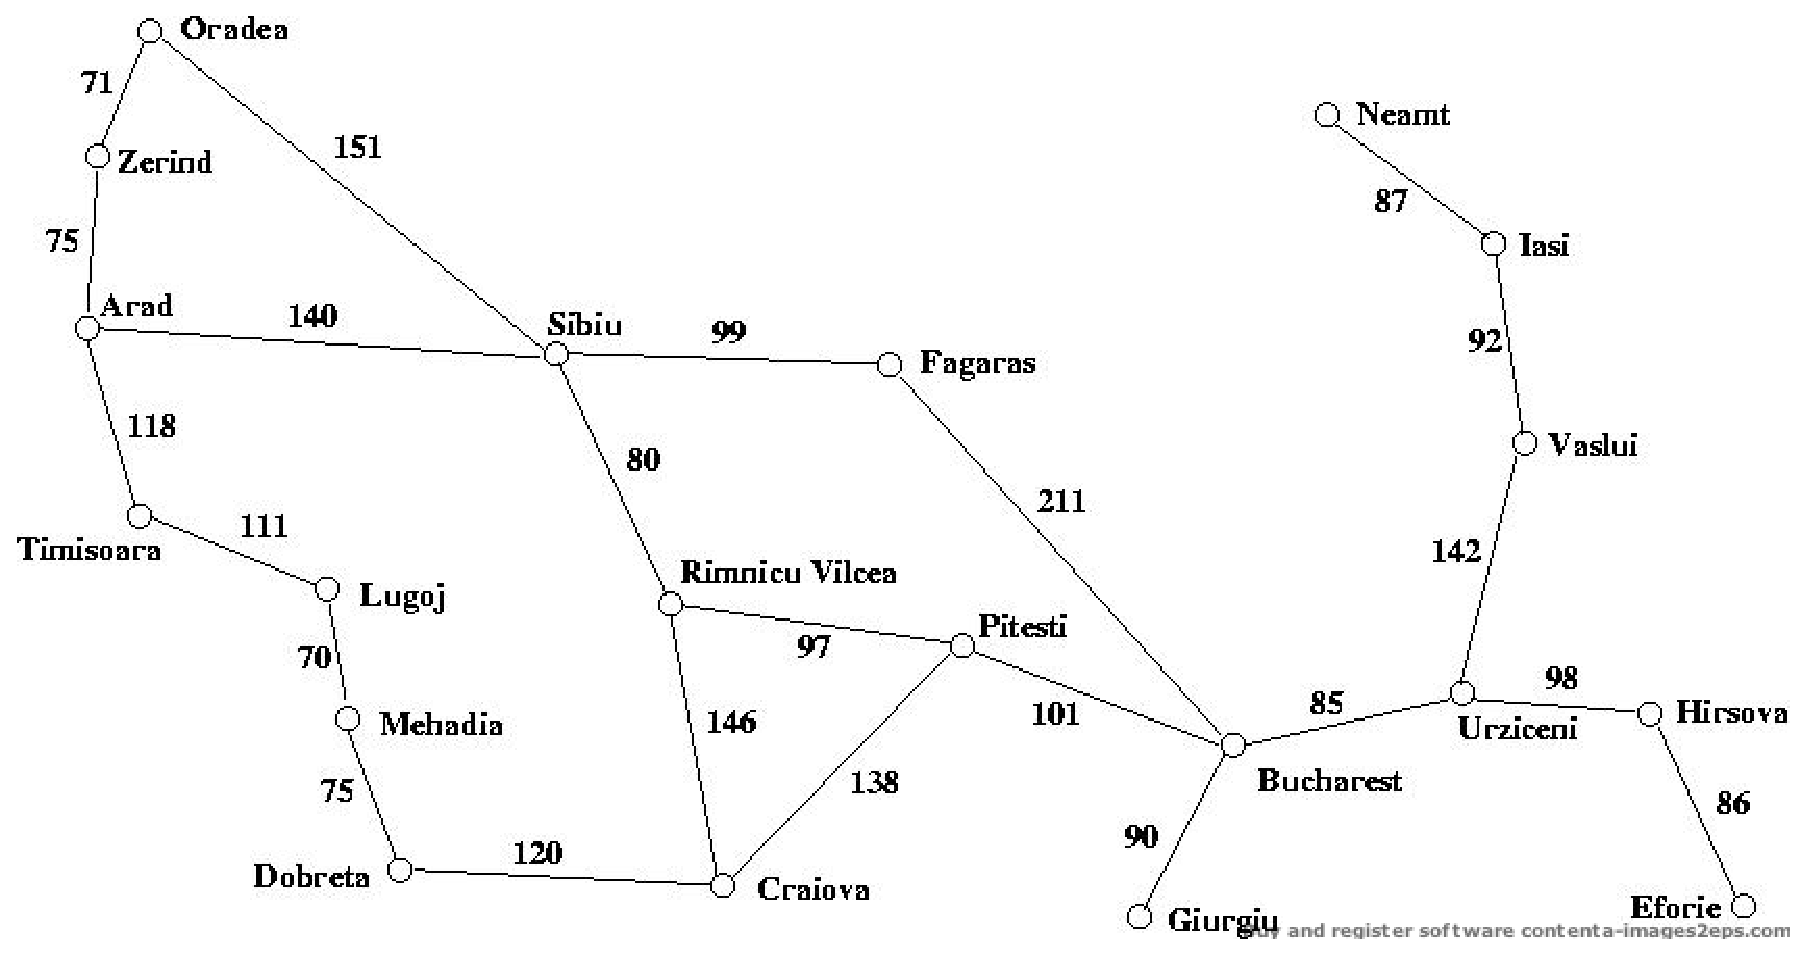
\includegraphics[scale=0.5, clip]{romania.eps} 
\vspace*{-2ex}
\end{figure}

For this assignment, you may use the Prolog source in the webnotes for dfs.pl, bfs2.pl and roads.pl. 

	\begin{enumerate}
	\item (8 points) Consider the path from Arad to Bucharest and the path from Bucharest to Arad. Show the paths returned by DFS and BFS results for each case.
Does either DFS or BFS return a path through the same set of cities for either? Give a reason for this behavior.
	\item (6 points) Is there a case where Depth-First performs worse than Breadth-First (in terms of number of cities visited in the path, not the distance) ? If yes, what is it? If not, explain why.
	\item (6 points) Is there a case where Breadth-First performs worse than Depth-First (in terms of number of cities visited in the path, not the distance)? If yes, what is it? If not, explain why.
	\item (10 points) For the same graph, perform a hand-execution of Depth-First Iterative Deepening (DFID) with increment and cutoff initialized to 1, starting at Oradea. List the nodes in the order expanded and the state of the datastructure for the first five iterations of DFID. Expand the nodes alphabetically and insert them in nondecreasing alphabetical order. Compare this list with Breadth-First Search. (No Prolog is required for the DFID portion of this question.).
	\end{enumerate}

\end{enumerate}
\end{document}
